\section{基于增量舒尔补的优化方法}

iSAM2算法\cite{kaess2008isam,kaess2012isam2}创新性地在SLAM问题中使用了贝叶斯树来编码集束优化过程中的信息矩阵分解过程,达到高效地更新平方根信息矩阵的目的,显著地提升了全局优化的性能。其算法不仅适用于SLAM中的集束优化问题,也适用于一般的非线性最小二乘问题。也正是为了保证通用性,iSAM2难以在状态之间的关联特点高度统一的SLAM问题中发挥更高的性能。

例如在图\ref{fig:sparse_matrix}中,正规方程的三维点部分(左上角部分)高度稀疏,呈对角块状,在求解时应该优先考虑这一部分的分解。iSAM2算法需要依赖COLAMD\citep{davis2004algorithm}算法来被动地检测矩阵分解的顺序,一方面需要额外的计算时间,另一方面也不一定能得到比经验更好的结果。

\subsection{舒尔补}

舒尔补(Schur complement)是一种常用的加速求解稀疏线性系统的方法,也特别适用于集束优化问题中的正规方程的求解。其本质上是基于高斯消元的分块求解线性系统的方法。对于一个集束优化问题,经过对调整变量的顺序,可以得到正规方程$\bm{\delta} =\Lambda\setminus\bm{\eta}$:
\begin{equation}
    \Lambda \doteq
    \begin{bmatrix}
        \mathrm{P} & \mathrm{W}^\top \\
        \mathrm{W} & \mathrm{C}
    \end{bmatrix};
    \quad
    \bm{\eta} \doteq
    \begin{bmatrix} \bm{\eta}_p \\ \bm{\eta}_c \end{bmatrix}
\end{equation}
其中$\mathrm{P}$是三维点状态对应的信息矩阵,$\mathrm{C}$是相机状态对应的信息矩阵,$\mathrm{W}$是三维点状态和相机状态的信息矩阵。求解三维点状态和相机状态之前,先通过行变换构建舒尔补方程:
\begin{equation}
    \begin{bmatrix}
        \mathrm{P} & \mathrm{W}^\top \\
                 0 & \mathrm{C}-\mathrm{W}\mathrm{P}^{-1}\mathrm{W}^\top
    \end{bmatrix}
    \begin{bmatrix} \bm{\delta}_p \\ \bm{\delta}_c \end{bmatrix} =
    \begin{bmatrix}
        \bm{\eta}_p \\
        \bm{\eta}_c-\mathrm{W}\mathrm{P}^{-1}\bm{\eta}_p
    \end{bmatrix}
    \label{eq:schur_complement}
\end{equation}
记舒尔补矩阵为$\mathrm{S}\doteq\mathrm{C}-\mathrm{W}\mathrm{P}^{-1}\mathrm{W}^\top$,右侧为$\bm{b}\doteq{\bm{\eta}_c-\mathrm{W}\mathrm{P}^{-1}\bm{\eta}_p}$。根据经验,集束优化问题中的三维点状态数量远多于相机状态数量,故矩阵$\mathrm{P}$的规模远大于舒尔补矩阵。通过求解下式
\begin{equation}
    \bm{\delta}_c = \mathrm{S} \enspace\setminus\enspace \bm{b}
    \label{eq:solve_schur}
\end{equation}
可以快速得到相机状态变量的值。又因为三维点之间没有直接通过因子相连,故其信息矩阵$\mathrm{P}$呈对角块稀疏状,如图\ref{fig:sparse_matrix}所示。因此$\mathrm{P}^{-1}$矩阵的计算往往非常快速,通过变量回代又可以高效地求解剩余变量:
\begin{equation}
    \bm{\delta}_p = \mathrm{P}
    \enspace\setminus\enspace
    \left( \bm{\eta}_p-\mathrm{W}^\top\bm{\delta}_c \right)
    \label{eq:back_sub}
\end{equation}

舒尔补虽然可以大幅加速集束优化的求解,但是在标准的集束优化算法中,每一轮迭代重新构建舒尔补方程的过程仍然需要耗费大量的时间。如前面提到的,SLAM问题具有很好的局部性,每一轮求解一般都只有一小部分较新的变量有所更新,如果采用增量式的方法,每一轮迭代时只重新计算这些变量在舒尔补方程中对应的部分,则可以进一步减少计算量。

\subsection{增量舒尔补}

\begin{figure}[htb!]
    \centering
    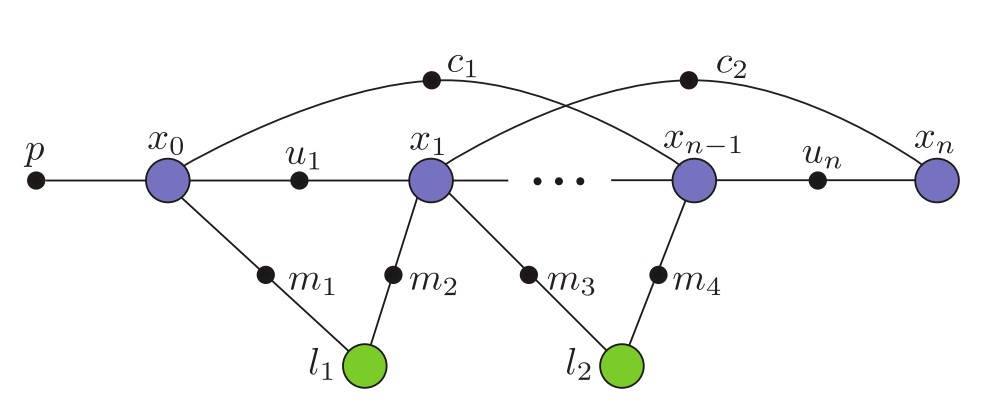
\includegraphics[width=.8\textwidth]{figs/factor_graph.png}
    \caption{因子图}
    \label{fig:factor_graph}
\end{figure}

如图\ref{fig:factor_graph}是一个常见集束优化问题的因子图示例,其对应的正规方程具有如图\ref{fig:normal_eq}所示的稀疏结构。按照式\eqref{eq:schur_complement}构建相机部分方程的舒尔补,依次迭代计算每一个三维点状态对应的舒尔补部分,并累加到图\ref{fig:reduced_sys}中的高亮部分所示的舒尔补中。图\ref{fig:schur_complement}展示了计算舒尔补的第一次迭代。

\begin{figure}[htb!]
    \centering
    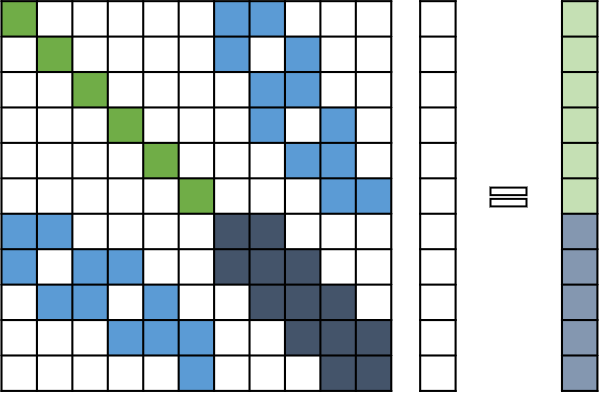
\includegraphics{figs/normal_eq.png}
    \caption{正规方程:左上角块对角矩阵部分对应三维点状态$1$至$6$的信息矩阵$\mathrm{P}$,右下角部分为相机状态$1$至$5$对应的信息矩阵$\mathrm{C}$,左下角和右上角为矩阵$\mathrm{W}$和$\mathrm{W}^\top$;中间列向量从上至下依次对应三维点状态$1$至$6$和相机状态$1$至$5$的迭代步;右侧部分从上至下依次对应三维点状态$1$至$6$和相机状态$1$至$5$。}
    \label{fig:normal_eq}
\end{figure}

\begin{figure}[htb!]
    \centering
    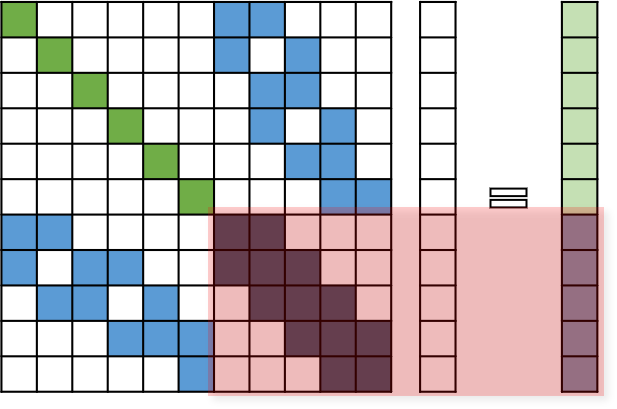
\includegraphics{figs/reduced_sys.png}
    \caption{舒尔补:高亮部分为相机状态对应舒尔补方程,其余部分为原方程。}
    \label{fig:reduced_sys}
\end{figure}

\begin{figure}[htb!]
    \centering
    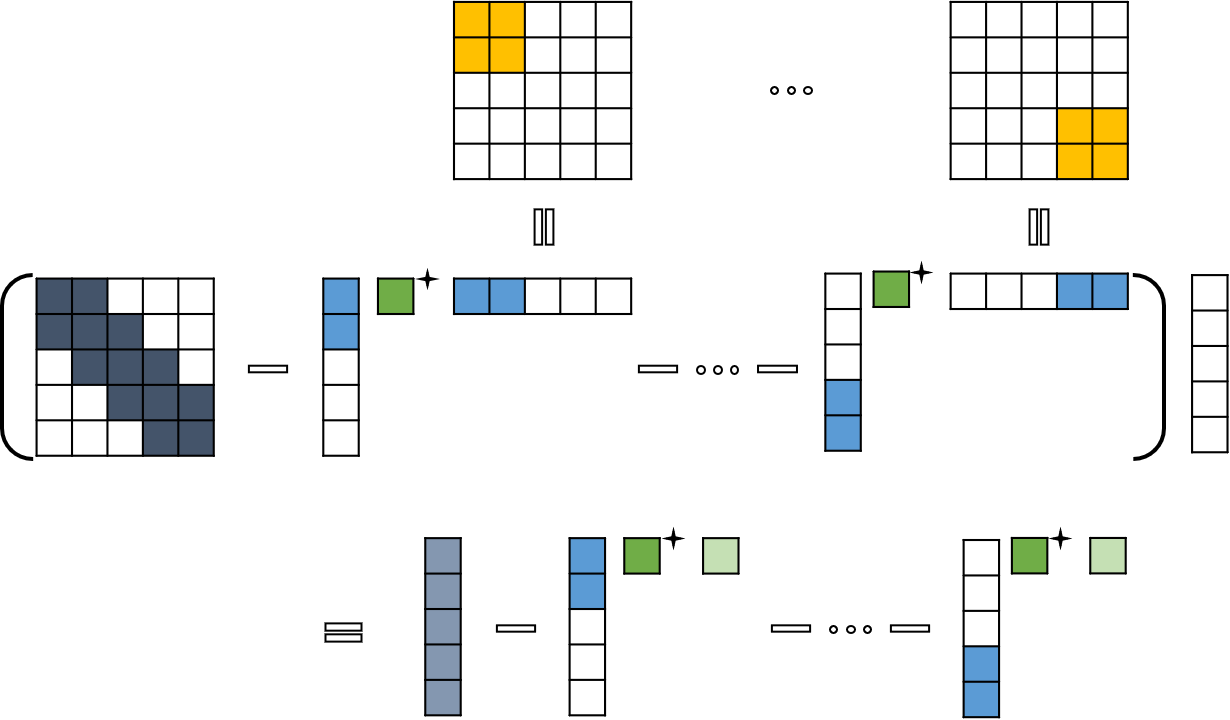
\includegraphics[width=\textwidth]{figs/schur_complement.png}
    \caption{计算舒尔补}
    \label{fig:schur_complement}
\end{figure}

\begin{figure}[htb!]
    \centering
    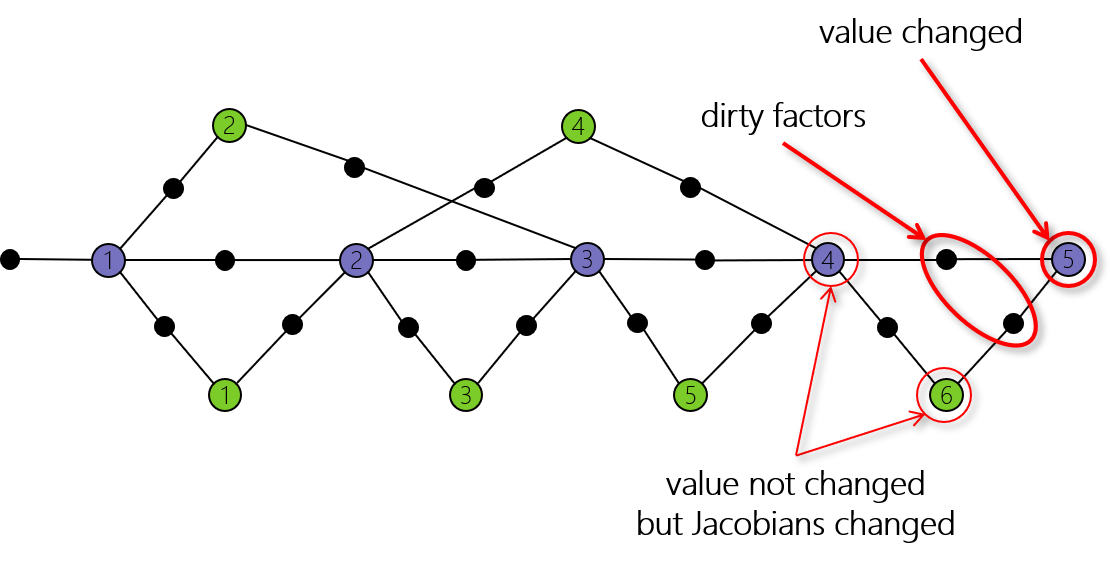
\includegraphics[width=.8\textwidth]{figs/factor_graph_dirty.png}
    \caption{因子图待更新部分:相机状态$5$为脏变量;与其直接相连的因子为脏因子;相机状态$4$和三维点状态$6$为只有梯度发生了变化的脏变量。}
    \label{fig:factor_graph_dirty}
\end{figure}

增量更新舒尔补的方法关键在于尽可能地复用上一次迭代的结果,只针对性地计算舒尔补方程中变化较大的变量对应的部分。以因子图\ref{fig:factor_graph}为例,假设只有相机状态$5$有较大的更新,则先将其标记为脏变量。在因子图中,只有与脏变量直接相连的因子需要标记为脏因子,如图\ref{fig:factor_graph_dirty}所示。需要注意的是,尽管相机状态$5$和三维点状态$6$的值并未发生足够大的改变,但是由于与之相邻的部分因子被标记为脏因子,因此也需要更新这些因子关于它们的雅各比矩阵。等价地,图\ref{fig:normal_eq_dirty}高亮展示了对应的舒尔补方程中需要更新的部分。

\begin{figure}[htb!]
    \centering
    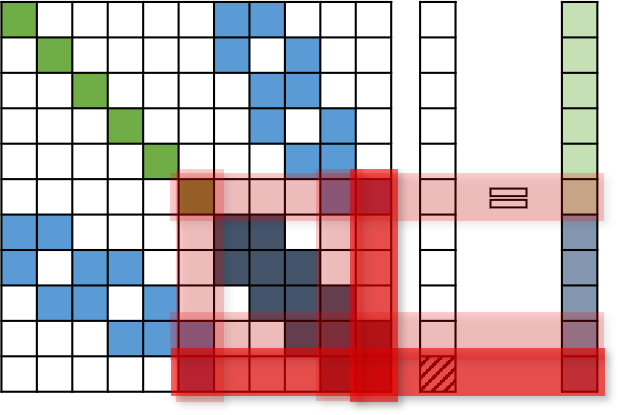
\includegraphics{figs/normal_eq_cursed.png}
    \caption{待更新舒尔补部分}
    \label{fig:normal_eq_dirty}
\end{figure}

\begin{figure}[htb!]
    \centering
    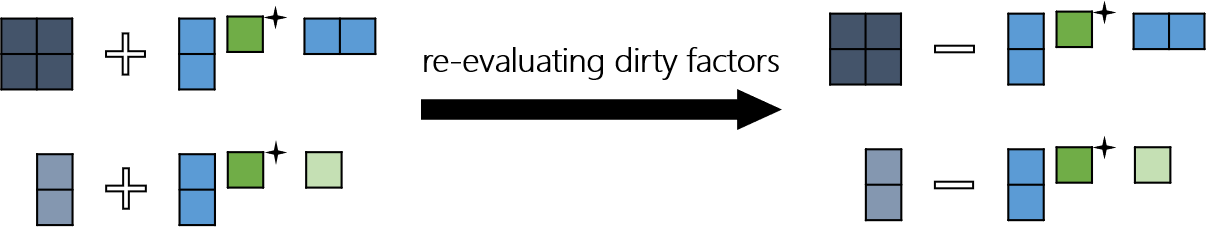
\includegraphics[width=\textwidth]{figs/schur_update.png}
    \caption{更新舒尔补}
\end{figure}

\begin{figure}[htb!]
    \centering
    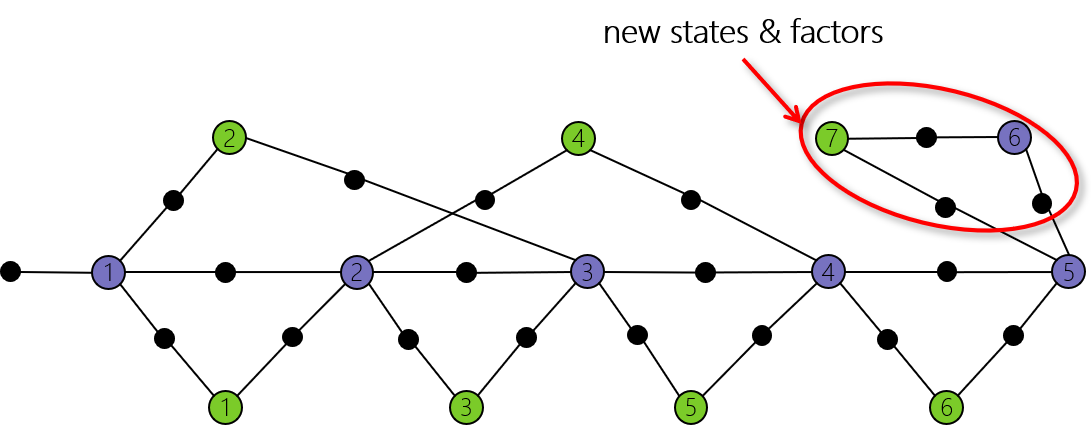
\includegraphics[width=.8\textwidth]{figs/factor_graph_aug.png}
    \caption{增广因子图}
\end{figure}

\begin{figure}[htb!]
    \centering
    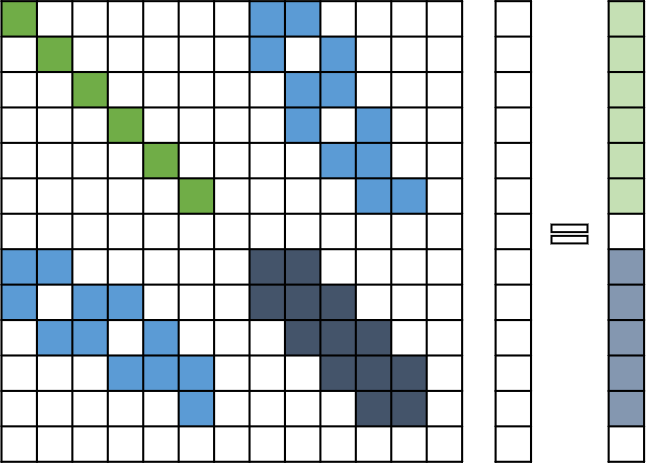
\includegraphics{figs/normal_eq_aug.png}
    \caption{增广正规方程}
\end{figure}

\begin{figure}[htb!]
    \centering
    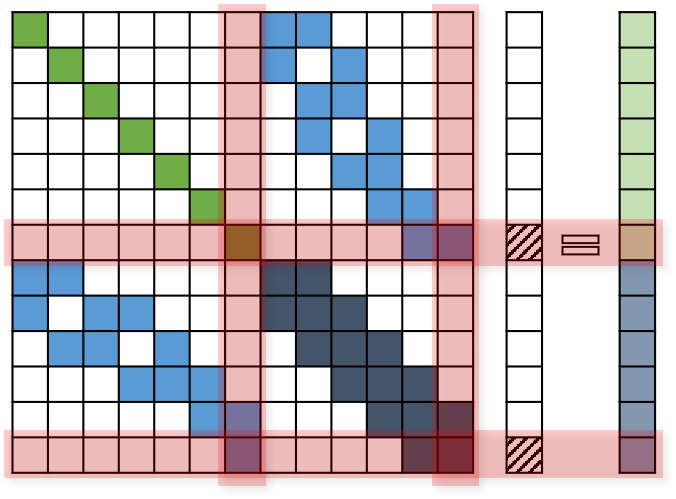
\includegraphics{figs/normal_eq_update.png}
    \caption{更新正规方程}
\end{figure}

\begin{figure}[htb!]
    \centering
    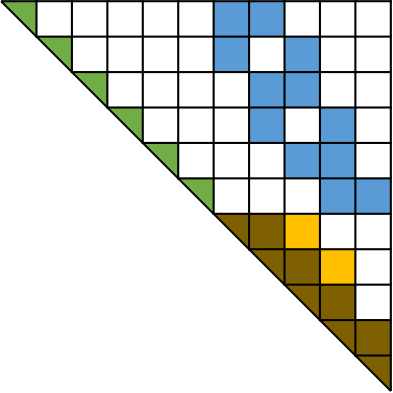
\includegraphics{figs/sqrt_info.png}
    \caption{平方根信息矩阵}
\end{figure}

\begin{figure}[htb!]
    \centering
    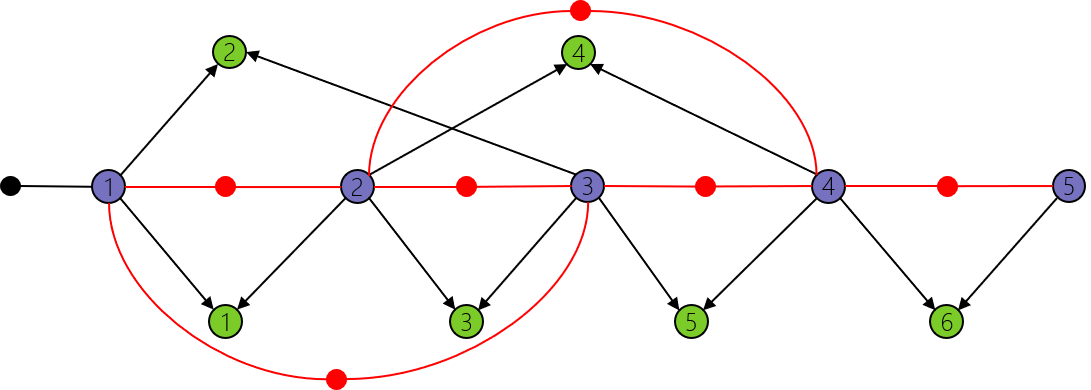
\includegraphics[width=.8\textwidth]{figs/elim.png}
    \caption{消元}
\end{figure}

\begin{figure}[htb!]
    \centering
    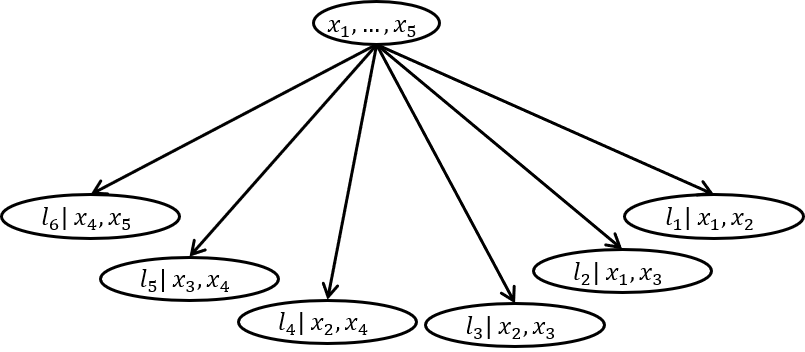
\includegraphics[width=\textwidth]{figs/bayes_tree.png}
    \caption{贝叶斯树}
\end{figure}

\begin{table}[htb!]
    \centering
    \caption{增量式集束优化算法对比:ICE-BA,SLAM++,iSAM2}
    \vspace{6pt}
    \begin{tabularx}{\textwidth}{c|X|X|X}
        \toprule
                        & \textbf{变量分组/排序} & \textbf{线性求解}            & \textbf{状态更新} \\ \hline
        \textbf{ICE-BA} & 三维点独立成组         & 增量舒尔补+松弛PCG           & 根据步长直接判断  \\ \hline
        \textbf{SLAM++} & 三维点独立成组         & 增量舒尔补+乔里斯基分解      & 根据步长直接判断  \\ \hline
        \textbf{iSAM2}  & CCOLAMD自动分组        & 基于贝叶树的即时线性化和求解 & 根据贝叶斯树推断  \\ \bottomrule
    \end{tabularx}
    \label{tab:comp}
\end{table}
